%
% $RCSfile: lifecycle.tex,v $
%
% Copyright (c) 2001-2004. Christian Heller. All rights reserved.
%
% No copying, altering, distribution or any other actions concerning this
% document, except after explicit permission by the author!
% At some later point in time, this document is planned to be put under
% the GNU FDL license. For now, _everything_ is _restricted_ by the author.
%
% http://www.cybop.net
% - Cybernetics Oriented Programming -
%
% http://www.resmedicinae.org
% - Information in Medicine -
%
% @author Christian Heller <christian.heller@tuxtax.de>
%

\section{An Extended Component Lifecycle}
\label{an_extended_component_lifecycle_heading}

The CYBOP lifecycle of components is an extension of the lifecycle idea of Apache
-- basically the same idea but another background and realization.\\
All \emph{Whole-Part associations} between objects were organized under the rules
of the component lifecycle. Analogous to the lifecycle of organic cells, the
relations were created and destroyed in a sequence of lifecycle steps. These
steps are realized as method calls on the components (figure
\ref{component_lifecycle_figure}).

\begin{figure}[ht]
    \begin{center}
       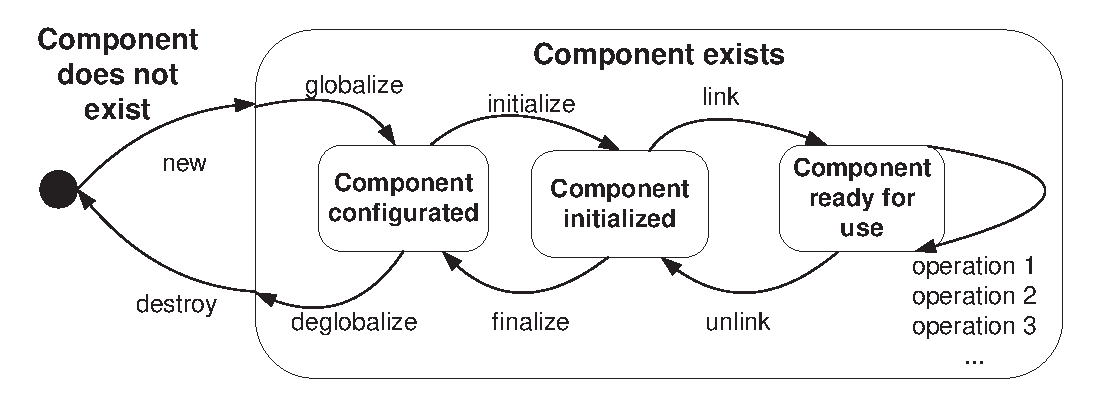
\includegraphics[scale=0.4]{eps/lebenszyklusEng.eps}
       \caption{State Diagram of CYBOB's Component Lifecycle}
       \label{component_lifecycle_figure}
    \end{center}
\end{figure}

